% ======================================================================
% Module 2: R0, equilibria and stability, final size, sensitivity
% Three frames, no title slide: \input this file into the main deck.
%
% Needs in the main preamble:  \usepackage{graphicx,booktabs,amssymb}
% Figures are in figs/ next to this file. If this file sits in a folder
% (e.g. module2/), add \graphicspath{{module2/}} to the main preamble.
% All numbers are from report/main.tex (final Colab run).
% ======================================================================

% Shared deck colours (same values as Modules 1 and 5)
\definecolor{mvPINN}{HTML}{7B2D8E}
\definecolor{mvInk}{HTML}{1F2933}
\definecolor{mvMuted}{HTML}{5F6B7A}
\definecolor{mvSoft}{HTML}{F3EDF6}
\definecolor{mvRule}{HTML}{C9B6D3}

\providecommand{\mvTakeaway}[1]{%
  \par\vspace{3pt}\noindent
  \fcolorbox{mvRule}{mvSoft}{\parbox{\dimexpr\linewidth-2\fboxsep-2\fboxrule\relax}{\footnotesize\color{mvInk}#1}}}

% ----------------------------------------------------------------------
\begin{frame}{$R_0$ and stability: will an outbreak grow?}
\framesubtitle{Module 2 \textbullet\ next-generation matrix, equilibria and the early growth rate (constant $\beta$)}
\vspace{-2pt}
\begin{columns}[T,onlytextwidth]
\column{0.50\textwidth}
  \footnotesize\raggedright
  \textbf{\color{mvPINN}Next-generation matrix}: split the $(e,i)$ equations into new infections $F$ and moves between classes $V$
  \[ F = \begin{pmatrix} 0 & \beta s^* \\ 0 & 0 \end{pmatrix},\quad
     V = \begin{pmatrix} \sigma & 0 \\ -\sigma & \gamma+\mu \end{pmatrix} \]
  \vspace{-8pt}
  \[ R_0 = \rho(FV^{-1})\ \text{at}\ s^* = 1\ =\ \frac{\beta}{\gamma+\mu} \]
  \vspace{-6pt}
  \begin{itemize}\setlength{\itemsep}{1pt}
    \item rate $\times$ time: $0.486$ /day $\times$ $4.1$ infectious days $\approx$ \textbf{2.00}
    \item $\sigma$ drops out: incubation changes \emph{when} people infect others, not \emph{how many}
    \item over time: $R_t = \beta(t)\,s(t)/(\gamma+\mu)$, which the PINN gives us
  \end{itemize}
  \vspace{3pt}
  \textbf{\color{mvPINN}Early growth rate} = the positive eigenvalue
  \[ \lambda_+ = 0.062734 \text{ /day (theory)}, \quad 0.062732 \text{ (simulation)} \]
  \vspace{-10pt}
  \begin{itemize}\setlength{\itemsep}{1pt}
    \item doubling time \textbf{11.1 days}; $R_0 = (1+\tfrac{\lambda_+}{\sigma})(1+\tfrac{\lambda_+}{\gamma+\mu})$ gives back 2.0004
  \end{itemize}
\column{0.46\textwidth}
  \footnotesize\raggedright
  \textbf{\color{mvPINN}Equilibria}: every one is disease-free, $(s^*, 0, 0, r^*, d^*)$\\
  {\scriptsize\color{mvMuted}no births and lasting immunity, so there is no endemic state}\\[3pt]
  \scriptsize\setlength{\tabcolsep}{5pt}
  \centering
  \begin{tabular}{@{}cccl@{}}
    \toprule
    $s^*$ & $R_0 s^*$ & eigenvalues ($e,i$ block) & result \\
    \midrule
    1.00 & 2.00 & $-0.412,\ \mathbf{+0.063}$ & unstable \\
    0.75 & 1.50 & $-0.383,\ \mathbf{+0.034}$ & unstable \\
    0.40 & 0.80 & $-0.334,\ -0.016$ & stable \\
    0.25 & 0.50 & $-0.307,\ -0.042$ & stable \\
    \bottomrule
  \end{tabular}\\[4pt]
  \raggedright\footnotesize
  \begin{itemize}\setlength{\itemsep}{1pt}
    \item threshold $R_0 s^* = 1$: herd immunity once $s^* < 1/R_0 = 50\%$
    \item \textbf{stable, not asymptotically}: three eigenvalues are 0, so the system settles at a \emph{nearby} disease-free state
  \end{itemize}
\end{columns}
\mvTakeaway{\textbf{One number decides growth:} a few infections grow if $R_0 s^* > 1$ and die out if $R_0 s^* < 1$.
The growth rate in early case data gives $R_0$ back, and our simulation matches the theory to $3\times10^{-5}$.}
\end{frame}

% ----------------------------------------------------------------------
\begin{frame}{Final size: how many people get infected in total?}
\framesubtitle{Module 2 \textbullet\ an exact answer without simulating, and a test for every numerical method in the project}
\vspace{-2pt}
\begin{columns}[T,onlytextwidth]
\column{0.40\textwidth}
  \footnotesize\raggedright
  \textbf{\color{mvPINN}Divide $\dot s$ by $\dot r + \dot d$: $i$ cancels}
  \[ \frac{ds}{d(r+d)} = \frac{-\beta s i}{(\gamma+\mu)\,i} = -R_0\, s \]
  \textbf{\color{mvPINN}Integrate to the end of the epidemic}
  \[ \ln\frac{s_0}{s_\infty} = R_0\,(1 - s_\infty - r_0 - d_0) \]
  \[ d_\infty = d_0 + \underbrace{\tfrac{\mu}{\gamma+\mu}}_{\text{CFR } 41\%}(1 - s_\infty - r_0 - d_0) \]
  \vspace{-4pt}
  \begin{itemize}\setlength{\itemsep}{1pt}
    \item $R_0 = 2$: \textbf{80\%} infected by the end, \textbf{33\%} die (no interventions)
    \item exactly one root in $(0, s_0)$; found with Brent's method
  \end{itemize}
\column{0.58\textwidth}
  \centering
  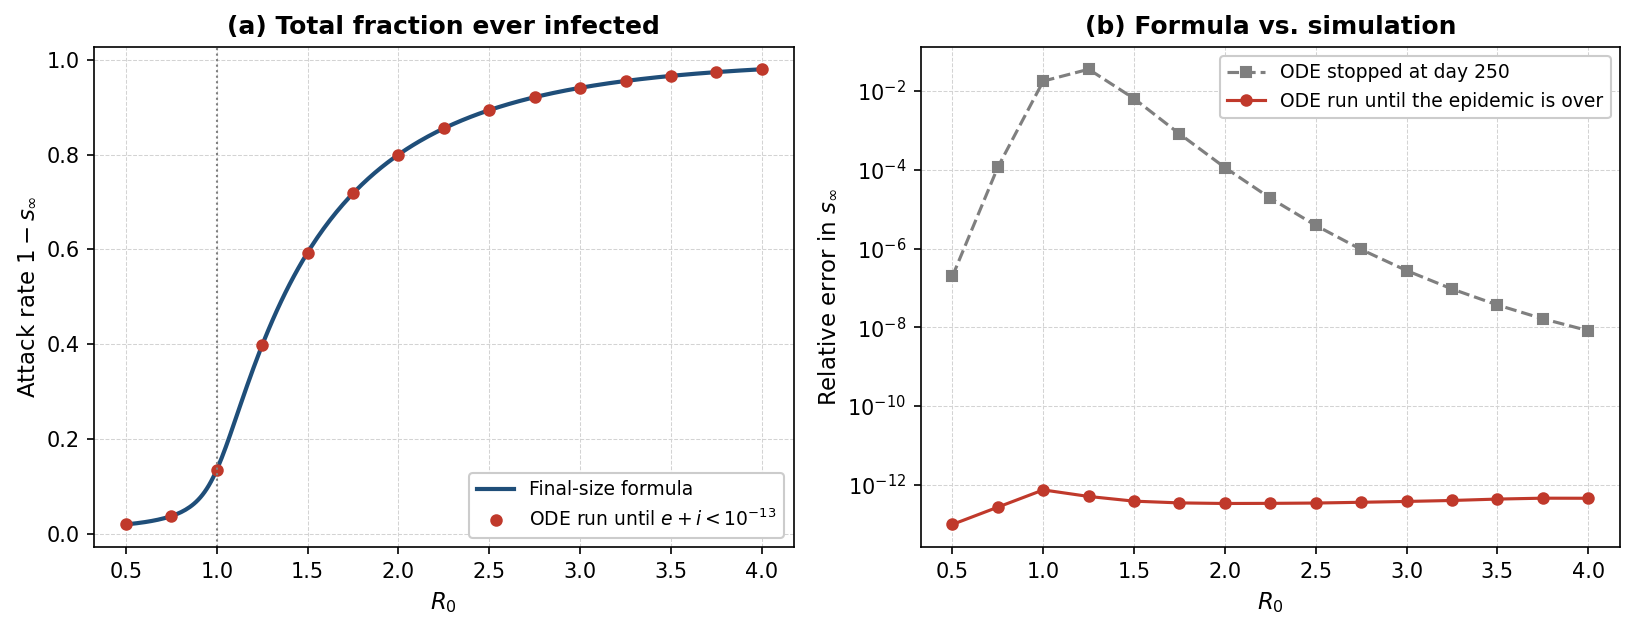
\includegraphics[width=\linewidth]{figs/m2_final_size.png}\\[1pt]
  \raggedright
  {\scriptsize\color{mvMuted}(a) formula (line) and ODE (dots); (b) error: run to the end (red) vs.\ stop at day 250 (grey)}\\[4pt]
  \footnotesize
  \begin{itemize}\setlength{\itemsep}{1pt}
    \item[$\checkmark$] run the ODE until $e+i<10^{-13}$: formula and ODE agree to $\mathbf{10^{-12}}$ for $R_0$ from 0.8 to 3.5
    \item[$\times$] stop at day 250: errors up to \textbf{3.6\%} near $R_0 = 1.25$, because slow epidemics last up to $\sim$1000 days
  \end{itemize}
\end{columns}
\mvTakeaway{\textbf{The catch:} the $\beta$ cancels only if it is constant. With $\beta(t)$ there is no closed formula,
which is one reason we need a data-driven method such as the PINN.}
\end{frame}

% ----------------------------------------------------------------------
\begin{frame}{Sensitivity: which parameters matter most?}
\framesubtitle{Module 2 \textbullet\ Latin hypercube sampling ($n = 1000$, seed 42) and partial rank correlation (PRCC)}
\vspace{-2pt}
\begin{columns}[T,onlytextwidth]
\column{0.49\textwidth}
  \centering
  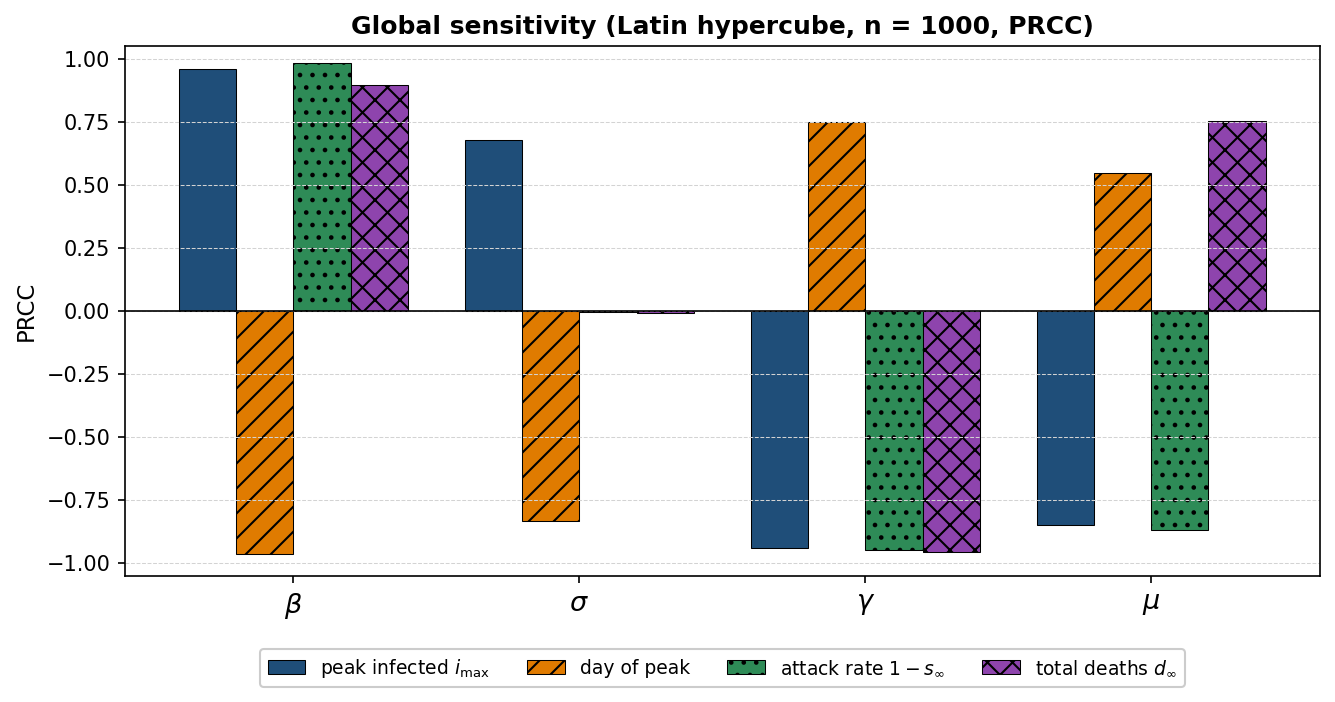
\includegraphics[width=\linewidth]{figs/m2_prcc.png}\\[1pt]
  {\scriptsize\color{mvMuted}PRCC = one parameter's effect with the others held fixed}
\column{0.48\textwidth}
  \scriptsize\setlength{\tabcolsep}{4pt}
  \centering
  \begin{tabular}{@{}lcccc@{}}
    \toprule
    & peak & peak day & attack rate & deaths \\
    \midrule
    $\beta$  & $+0.96$ & $-0.96$ & $+0.98$ & $+0.90$ \\
    $\sigma$ & $+0.68$ & $-0.83$ & $0.00$\textsuperscript{n.s.} & $-0.01$\textsuperscript{n.s.} \\
    $\gamma$ & $-0.94$ & $+0.75$ & $-0.95$ & $-0.95$ \\
    $\mu$    & $-0.85$ & $+0.55$ & $-0.87$ & $+0.75$ \\
    \bottomrule
  \end{tabular}\\[1pt]
  \raggedright
  {\tiny\color{mvMuted}\textsuperscript{n.s.} not significant at the 1\% level.\\ Local index of $R_0$ (\% change per 1\%): $\beta$ $+1$, $\gamma$ $-0.59$, $\mu$ $-0.41$, $\sigma$ 0.}\\[4pt]
  \footnotesize
  \begin{itemize}\setlength{\itemsep}{1pt}
    \item $\beta$ raises everything: the main lever for control
    \item $\gamma$, $\mu$ shrink the epidemic, but $\mu$ \textbf{raises} deaths
    \item $\sigma$ moves the peak but not the final size, \textbf{as the formula predicts}
  \end{itemize}
\end{columns}
\mvTakeaway{\textbf{What this means for the PINN:} cases and deaths alone cannot separate $\sigma$, $\gamma$ and $\mu$.
So we fix $\sigma$ and $\gamma$ from clinical data; the PINN learns $\beta(t)$, and $\mu$ from the share of cases that die.}
\end{frame}
